% Compile on Overleaf: pdfLaTeX (or LuaLaTeX).
% Short PPT-style summary of the Milvus GPU to AMD (HIP) port.
\documentclass[aspectratio=169,11pt]{beamer}

\usetheme{Madrid}
\usecolortheme{whale}
\setbeamertemplate{navigation symbols}{}
\setbeamertemplate{footline}[frame number]
\setbeamerfont{title}{size=\Large\bfseries}
\setbeamerfont{frametitle}{size=\large\bfseries}

\usepackage{booktabs}
\usepackage{array}
\usepackage{tikz}
\usepackage{hyperref}
\usetikzlibrary{arrows.meta,shapes.geometric}

\title{Porting Milvus GPU Vector Search to AMD}
\subtitle{HIP / hipVS / Knowhere --- lab results on RX 7900 XTX}
\author{Konstantin Kolchin}
\date{July 2026}

\begin{document}

%----- 1 -----
\begin{frame}[fragile]
  \titlepage
  \vspace{0.4em}
  \begin{center}
    \small
    Developed with \textbf{Cursor} + \textbf{Grok 4.5} agent assistance.\\[0.4em]
    \textbf{Actual calendar:} about \textbf{2 weeks}
    \quad|\quad
    \textbf{Estimate without this assistance:} \textbf{6--8 weeks}.
  \end{center}
\end{frame}

%----- 2 -----
\begin{frame}{Goal}
  \begin{block}{Project objective}
    Replace the NVIDIA \textbf{cuVS / cuRAFT} path in Milvus with AMD
    \textbf{hipVS / hipRAFT} (ROCm), so sealed GPU ANN indexes run on Radeon GPUs.
  \end{block}

  \vspace{0.5em}
  \begin{columns}[T]
    \begin{column}{0.48\textwidth}
      \textbf{Stack}
      \begin{itemize}
        \item pymilvus / clients
        \item Milvus server
        \item Knowhere (GPU indexes)
        \item hipVS + hipRAFT (AMD)
      \end{itemize}
    \end{column}
    \begin{column}{0.48\textwidth}
      \textbf{Primary target}
      \begin{itemize}
        \item Index: \texttt{GPU\_IVF\_FLAT}
        \item Host: RX 7900 XTX (\texttt{gfx1100})
        \item Line: Milvus \texttt{v2.5.4}
        \item Control: CPU Milvus (same host)
      \end{itemize}
    \end{column}
  \end{columns}
\end{frame}

%----- 3 -----
\begin{frame}{Approach: five layers}
  \begin{enumerate}
    \item[\textbf{0}] ROCm + CPU Milvus sanity
    \item[\textbf{1}] hipRAFT / hipVS alone (+ IVF packer fix on gfx1100)
    \item[\textbf{2}] Knowhere + HIP (DXC \texttt{knowhere} \texttt{2.5})
    \item[\textbf{3}] Milvus source + sealed GPU build/load
    \item[\textbf{4}] Full SIFT-1M harness: recall + QPS vs CPU Milvus
  \end{enumerate}

  \vspace{0.6em}
  \begin{exampleblock}{Status (2026-07-17)}
    Layers \textbf{0--4 complete} on the lab host.\\
    DXC: Knowhere \texttt{2.5} + Milvus \texttt{v2.5.4} HIP line merged.\\
    Delivery: about 2 weeks with Cursor + Grok 4.5 (vs 6--8 weeks without).
  \end{exampleblock}
\end{frame}

%----- 4 -----
\begin{frame}[fragile]{How vector search works (end to end)}
  \begin{columns}[T]
    \begin{column}{0.48\textwidth}
      \textbf{Procedure}
      \begin{enumerate}
        \item \textbf{Store} many vectors in the database
              (here: 1M image descriptors).
        \item \textbf{Query} arrives: one new vector
              (``find items like this'').
        \item Engine finds the \textbf{k nearest}
              stored vectors (we use $k=10$).
        \item Returns their IDs (and distances)
              to the application.
      \end{enumerate}
      \vspace{0.3em}
      {\small Exact scan of 1M vectors is slow;
      IVF + GPU approximates this fast.}
    \end{column}
    \begin{column}{0.50\textwidth}
      \centering
      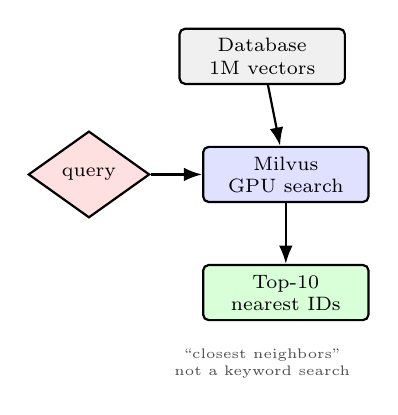
\begin{tikzpicture}[
        font=\scriptsize,
        box/.style={draw, rounded corners=2pt, align=center,
                    minimum width=2.1cm, minimum height=0.7cm, thick},
        arr/.style={-{Latex}, thick}
      ]
        \node[box, fill=gray!12] (db) at (0,2.6)
          {Database\\1M vectors};
        \node[draw, diamond, aspect=1.6, fill=red!12, thick,
              align=center, minimum size=1.1cm]
          (q) at (-2.2,1.1) {query};
        \node[box, fill=blue!12] (eng) at (0.3,1.1)
          {Milvus\\GPU search};
        \node[box, fill=green!15] (out) at (0.3,-0.4)
          {Top-10\\nearest IDs};

        \draw[arr] (db) -- (eng);
        \draw[arr] (q) -- (eng);
        \draw[arr] (eng) -- (out);

        \node[font=\tiny, text=black!70, align=center]
          at (0,-1.3) {``closest neighbors''\\not a keyword search};
      \end{tikzpicture}
    \end{column}
  \end{columns}
\end{frame}

%----- 5a -----
\begin{frame}{Two fair compares (do not mix them)}
  \footnotesize
  \textbf{Why VectorDBBench looked ``slow'' on GPU:} our sweep used
  \texttt{--search-serial} (one query RPC at a time) to measure latency + recall.
  That under-uses a GPU. Throughput needs a \textbf{batched} client.\\[0.4em]

  \begin{tabular}{@{}p{0.22\textwidth}p{0.35\textwidth}p{0.35\textwidth}@{}}
    \toprule
    & \textbf{A --- VDBBench serial} & \textbf{B --- Batched harness} \\
    \midrule
    Client & 1 query / RPC & 10k queries / \texttt{search()} \\
    Shows & Correctness, single-query latency & Throughput (where GPU wins) \\
    Management lead? & No (appendix) & \textbf{Yes} \\
    \bottomrule
  \end{tabular}

  \vspace{0.5em}
  Sealed path confirmed on both: IndexNode/QueryNode \texttt{GPU\_CUVS\_IVF\_FLAT},
  no \texttt{InvalidDeviceFunction}.
\end{frame}

%----- 5b -----
\begin{frame}{A --- VDBBench serial (latency protocol)}
  \footnotesize
  Same host, SIFT-1M, \texttt{nlist}=1024, \texttt{k}=10 (2026-07-18).\\
  Both: VectorDBBench \texttt{--search-serial}. Speed-up $=$ GPU/CPU QPS.\\[0.25em]

  \begin{center}
  \begin{tabular}{@{}lrrrr@{}}
    \toprule
    \textbf{nprobe} & \textbf{CPU QPS} & \textbf{GPU QPS} & \textbf{R@10} & \textbf{Speed-up} \\
    \midrule
    1  & 1575 & 418 & $\approx0.38$ & $0.27\times$ \\
    4  & 1211 & 412 & $\approx0.71$ & $0.34\times$ \\
    8  &  924 & 345 & $\approx0.84$ & $0.37\times$ \\
    16 &  626 & 676 & $0.931$ & $1.08\times$ \\
    32 &  371 & 773 & $0.979$ & $2.08\times$ \\
    \bottomrule
  \end{tabular}
  \end{center}

  \vspace{0.3em}
  \textbf{Takeaway:} recall ladders match (port correctness). Not the GPU throughput story.
\end{frame}

%----- 5c -----
\begin{frame}{B --- Batched search (throughput --- lead with this)}
  \footnotesize
  Same host, SIFT-1M, \texttt{nlist}=1024, \texttt{k}=10.\\
  \textbf{Both} use one \texttt{search()} with all 10k queries
  (CPU: \texttt{run\_milvus\_hdf5.py IVF\_FLAT}; GPU: Layer-4
  \texttt{GPU\_IVF\_FLAT}).\\[0.25em]

  \begin{center}
  \begin{tabular}{@{}lrrrr@{}}
    \toprule
    \textbf{nprobe} & \textbf{CPU QPS} & \textbf{GPU QPS} & \textbf{R@10 (GPU)} & \textbf{Speed-up} \\
    \midrule
    1  & 22013$^\dagger$ & 16982 & 0.382 & $0.77\times$ \\
    4  & 14509$^\dagger$ & 21882 & 0.709 & $1.51\times$ \\
    8  &  9516$^\dagger$ & 21838 & 0.844 & $2.30\times$ \\
    16 &  5402$^\dagger$ & 26181 & 0.934 & $4.85\times$ \\
    32 &  2749$^\dagger$ & 19578 & 0.980 & $7.12\times$ \\
    \bottomrule
  \end{tabular}
  \end{center}

  \vspace{0.25em}
  {\scriptsize $^\dagger$CPU from same-host batched diagnostic (runbook Table~7, Jul~7);
  GPU = Layer-4 harness Jul~17. Re-run CPU with
  \texttt{scripts/run\_milvus\_batch\_cpu\_compare.sh} on Docker v2.5.4 for strict parity.}

  \vspace{0.2em}
  \textbf{Takeaway:} at production-like \texttt{nprobe} (16--32), GPU HIP is
  $\sim$5--7$\times$ CPU on the same batch protocol; sealed \texttt{GPU\_CUVS\_IVF\_FLAT}.
\end{frame}

%----- 6 -----
\begin{frame}[fragile]{What is recall@10?}
  \begin{columns}[T]
    \begin{column}{0.50\textwidth}
      \textbf{In one sentence}
      \begin{itemize}
        \item For each query we know the
              \emph{true} 10 nearest neighbors
              (from a trusted ground truth).
        \item The system also returns 10 IDs.
        \item \textbf{recall@10} = fraction of the
              true top-10 that appear in the
              system's top-10.
      \end{itemize}
      \vspace{0.35em}
      \textbf{Example:} true top-10 has 10 IDs;
      system finds 8 of them $\rightarrow$
      recall@10 $= 0.8$ (80\%).
      \vspace{0.35em}

      {\small $1.0$ = perfect; lower = more misses.\\
      Our GPU table goes about $0.38 \rightarrow 0.98$
      as search gets more thorough.}
    \end{column}
    \begin{column}{0.48\textwidth}
      \centering
      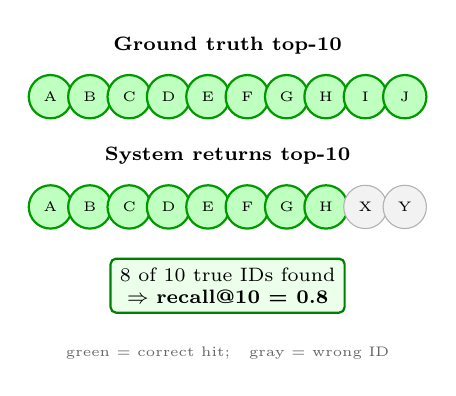
\begin{tikzpicture}[
        font=\tiny,
        hit/.style={circle, draw=green!60!black, fill=green!25,
                    minimum size=0.55cm, thick},
        miss/.style={circle, draw=red!70!black, fill=red!15,
                     minimum size=0.55cm, thick},
        other/.style={circle, draw=gray!60, fill=gray!10,
                      minimum size=0.55cm},
      ]
        \node[font=\scriptsize\bfseries] at (0,2.35) {Ground truth top-10};
        \foreach \i/\lab in {0/A,1/B,2/C,3/D,4/E,5/F,6/G,7/H,8/I,9/J} {
          \node[hit] at (-2.25+0.5*\i,1.7) {\lab};
        }

        \node[font=\scriptsize\bfseries] at (0,0.95) {System returns top-10};
        \foreach \i/\lab/\sty in {
          0/A/hit,1/B/hit,2/C/hit,3/D/hit,4/E/hit,
          5/F/hit,6/G/hit,7/H/hit,8/X/other,9/Y/other} {
          \node[\sty] at (-2.25+0.5*\i,0.3) {\lab};
        }

        \node[draw=green!50!black, thick, rounded corners=2pt,
              fill=green!8, align=center, font=\scriptsize]
          at (0,-0.7)
          {8 of 10 true IDs found\\
           $\Rightarrow$ \textbf{recall@10 = 0.8}};

        \node[font=\tiny, text=black!60, align=left]
          at (0,-1.55)
          {green = correct hit;\quad gray = wrong ID};
      \end{tikzpicture}
    \end{column}
  \end{columns}
\end{frame}

%----- 7 -----
\begin{frame}[fragile]{What is nprobe? (IVF search knob)}
  \begin{columns}[T]
    \begin{column}{0.52\textwidth}
      \textbf{IVF idea (plain language)}
      \begin{itemize}
        \item Vectors are grouped into many
              \emph{lists} (clusters). We used
              \texttt{nlist}=1024 lists.
        \item A query first finds the
              \emph{nearest list centers}.
        \item Then it searches only inside
              \textbf{nprobe} of those lists
              --- not the whole database.
      \end{itemize}
      \vspace{0.4em}
      \textbf{Trade-off}
      \begin{itemize}
        \item Higher \texttt{nprobe}: better recall, more work (usually lower QPS).
        \item Lower \texttt{nprobe}: faster, may miss true neighbors.
      \end{itemize}
    \end{column}
    \begin{column}{0.46\textwidth}
      \centering
      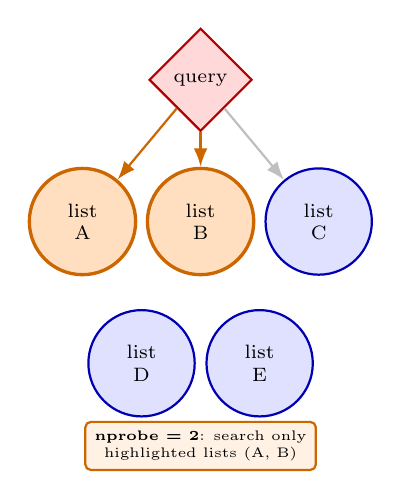
\begin{tikzpicture}[
        font=\scriptsize,
        list/.style={circle, draw=blue!70!black, fill=blue!12,
                     minimum size=1.35cm, align=center, thick},
        probed/.style={circle, draw=orange!80!black, fill=orange!25,
                       minimum size=1.35cm, align=center, very thick},
        qry/.style={diamond, draw=red!70!black, fill=red!15,
                    minimum size=0.85cm, align=center, thick},
        arr/.style={-{Latex}, thick}
      ]
        \node[qry] (Q) at (0,2.1) {query};
        \node[probed] (L1) at (-1.5,0.3) {list\\A};
        \node[probed] (L2) at (0.0,0.3) {list\\B};
        \node[list]   (L3) at (1.5,0.3) {list\\C};
        \node[list]   (L4) at (-0.75,-1.5) {list\\D};
        \node[list]   (L5) at (0.75,-1.5) {list\\E};

        \draw[arr, orange!80!black] (Q) -- (L1);
        \draw[arr, orange!80!black] (Q) -- (L2);
        \draw[arr, gray!50] (Q) -- (L3);

        \node[draw=orange!80!black, thick, rounded corners=2pt,
              fill=orange!10, align=center, font=\tiny]
          at (0,-2.55)
          {\textbf{nprobe = 2}: search only\\highlighted lists (A, B)};
      \end{tikzpicture}
    \end{column}
  \end{columns}
\end{frame}

%----- 8 -----
\begin{frame}{Where it lives and next steps}
  \begin{block}{Repositories (use v2.5.4, not amd/main)}
    \begin{itemize}
      \item Milvus HIP: \texttt{github.dxc.com/llmkb-internal/milvus} $\rightarrow$ \textbf{v2.5.4}
      \item Knowhere HIP: \texttt{github.dxc.com/llmkb-internal/knowhere} $\rightarrow$ \textbf{2.5}
      \item Harness / docs: \texttt{github.com/konkolchin/ann-harness-amd}
            (\texttt{docs/readme.txt}, porting plan PDF)
    \end{itemize}
  \end{block}

  \begin{columns}[T]
    \begin{column}{0.55\textwidth}
      \begin{block}{Next}
        \begin{itemize}
          \item Coworker rebuild + HIP vs \textbf{CUDA Milvus} (v2.5.4)
          \item Optional: IVF\_PQ / CAGRA; later public GitHub port
        \end{itemize}
      \end{block}
    \end{column}
    \begin{column}{0.42\textwidth}
      \begin{block}{Delivery note}
        Cursor + \textbf{Grok 4.5} agent:\\
        about 2 weeks actual vs\\
        6--8 weeks without.
      \end{block}
    \end{column}
  \end{columns}
\end{frame}

\end{document}
